\documentclass[10pt]{article}
\usepackage[utf8]{inputenc}
\usepackage[T1]{fontenc}
\usepackage{amsmath}
\usepackage{amsfonts}
\usepackage{mathrsfs}
\usepackage{amssymb}
\usepackage[version=4]{mhchem}
\usepackage{stmaryrd}
\usepackage{bbold}
\usepackage{enumitem}
\usepackage{hanging} %reference indent
\usepackage[a4paper,left=25mm,right=25mm,top=40mm,bottom=40mm]{geometry}
\usepackage{sectsty}
\sectionfont{\fontsize{10}{15}\selectfont}
\subsectionfont{\fontsize{10}{15}}
\usepackage[mathlines,switch]{lineno}
\usepackage{amsthm}
\usepackage{kotex}
\usepackage{xcolor}
\usepackage{graphicx} % insert image
\usepackage{multicol} % multi column
\usepackage{algorithm}
\usepackage{algpseudocode}
\usepackage{float}
\usepackage{tabularx}
\usepackage{multirow} % multirow in table
\usepackage{tikz}
\usepackage{subcaption}
\usepackage{hyperref}
\modulolinenumbers[5]
% \linenumbers

\usepackage{titlesec}
\titleformat{\section}
{\normalfont\fontsize{12}{12}\bfseries}{\thesection}{1em}{}
\titleformat{\subsection}
{\normalfont\fontsize{11}{11}\bfseries}{\thesubsection}{1em}{}
\titlespacing{\paragraph}{0pt}{\parskip}{5pt}
\titleformat{\title}
{\normalfont\fontsize{13}{13}\bfseries}{\thetitle}{1em}{}

\usepackage{indentfirst} % first line indent
\setlength{\parindent}{10pt}

\renewcommand{\arraystretch}{1.1}

\title{
\textbf{Learning semi-Markovian DAGs with flow-based VAE}}

\author{\normalsize\bfseries Dangchan Kim, Byungguk Kang, Jaeseok Kim, Minchan Kim}

\begin{document}
\maketitle

\begin{abstract}
    We propose a method to learn the structure of a semi-Markovian directed acyclic graph, which is a mixed graph containing both directed and bidirectional edges, using a flow-based variational autoencoder. The proposed method is based on the assumption that noise variables in the linear structural equation model can be considered as latent variables. To learn the structure of the mixed graph, we employ an inverse autoregressive flow to approximate the dependency structure of the noise variables and its prior distribution. We conducted experiments on simulated data by adjusting the number of nodes and the proportion of bidirectional edges. The code is available at \url{https://github.io/ddangchani/NFG-VAE}.
\end{abstract}

\section{Introduction}

Directed acyclic graphs (DAGs) are commonly used to represent causal relationships between variables \cite{pearl_2009}. However, recovering the causal structure from observational data is an NP-hard problem \cite{ChickeringNPhard}. To overcome this problem, several methods have been proposed. NOTEARS \cite{zheng2018dags} is a method that learns the structure of DAGs by minimizing the continuous approximation of the discrete constraint, enabling the learning of DAGs through continuous optimization.\\

Based on the continuous acyclicity constraint neural network-based approaches known as graph neural networks, have been proposed. \cite{yu2019daggnn,li2020dirichlet,kipf2016variational,zhang2019dvae} The most representative model would be DAG-GNN \cite{yu2019daggnn}, a method that learns the structure of DAGs by using a neural network that takes the adjacency matrix of the graph as an additional input. It utilizes a variational autoencoder (VAE) to learn DAGs by interpreting the noise variable in the linear structural equation model as a latent variable.\\

However, in some cases, the noise variables may not be independent. For example, in a linear structural equation model with correlated hidden variables, the noise variables may exhibit a dependency structure. In such cases, edges with correlation in the noise variable are considered bidirectional edges, and these models are referred to as semi-Markovian \cite{Shipster2006semimarkovian}. Since the prior distribution of the noise variable is assumed to be a standard Gaussian in DAG-GNN or other graph neural networks, it becomes challenging to learn the structure of semi-Markovian DAGs. Therefore, we propose a method to learn the full covariance matrix of the noise variable using a flow-based VAE.

\section{Directed Acyclic Graphs and Mixed Graphs}
\subsection{Directed Acyclic Graphs}

Here is the introduction of DAGs

\subsection{Mixed Graphs}

Here is the introduction of mixed graphs

\subsection{Graph Learning}

Here is the introduction of graph learning

\section{Variational Autoencoders and Normalizing Flows}

\subsection{Variational Autoencoders}

Here is the introduction of VAEs

\subsection{Normalizing Flows}

Normalizing flows are a method of transforming a simple distribution into a complex distribution \cite{rezende15normalizingflows}. Let $z$ be a random variable with a simple distribution $p(z)$, and $x$ be a random variable with a complex distribution $p(x)$. We can transform $z$ into $x$ using a series of invertible transformations $\{f_k\}_{k=1,\ldots,T}$ as follows:
\begin{equation}
    x = f_T \circ f_{T-1} \circ \cdots \circ f_1(z)
\end{equation}

The probability density function of $x$ can be obtained by the change of variables formula:
\begin{equation}
    p(x) = p(z) \left| \det \left( \frac{\partial f_T \circ f_{T-1} \circ \cdots \circ f_1(z)}{\partial z} \right) \right|
\end{equation}

In VAE, the prior distribution of the latent variable $\mathbf{z}$ is typically assumed to be a standard Gaussian distribution or a multivariate Gaussian distribution with a diagonal covariance matrix. \cite{kingma2013auto} However, to employ a more flexible prior distribution, we can utilize normalizing flows to transform the standard Gaussian distribution into a more complex distribution. This allows us to capture richer and more intricate patterns in the latent space, such as correlation between latent variables.\\

There are several types of normalizing flows, such as Householder flow \cite{tomczak2017householder}, planar flow \cite{rezende15normalizingflows}, etc. In this paper, we use the inverse autoregressive flow (IAF) \cite{kingma2016iaf}, especially linear IAF. The linear IAF is defined as follows:

\begin{equation}
    \bf z_t = \bf \mu_t + \bf \sigma_t \odot \bf z_{t-1}.
\end{equation}

The linear IAF is the simplest case of IAF, which transforms a multivariate Gaussian with diagonal covariance to a multivariate Gaussian with full covariance. The transformation is invertible and the determinant of the Jacobian is easily computable. To use linear IAF at VAE, we need to produce an extra output $\mathbf{L(x)}$ from the encoder network. The full-covariance Gaussian distribution is obtained by the following transformation:

\begin{equation}
    \mathbf{z}_T = \mathbf{L(x)} \cdot \mathbf{z}_0.
\end{equation}

Note if we restrict the $\mathbf{L(x)}$ to be a lower triangular matrix with diagonal elements of ones, then the log-determinant of the Jacobian is zero, which is so-called volume preserving normalizing flow. \cite{kingma2016iaf}\\

With the linear IAF, the KL loss term can be written in closed form as follows:
\begin{equation}
    \begin{aligned}
        D_{KL}(q_\phi(\mathbf{z}_0 | \mathbf{x}) \Vert p(\mathbf{z}_T)) &=
        \log q_\phi(\mathbf{z}_0 | \mathbf{x}) - \log p(\mathbf{z}_T) \\
        &= -\frac{1}{2}(\mathbf{z}_0 -\mu_\phi)^T\Sigma_\phi^{-1}(\mathbf{z}_0 -\mu_\phi) + \frac{1}{2}\mathbf{z}_T^T\mathbf{z}_T \\
    \end{aligned}
\end{equation}

where $\mu_\phi$ and $\Sigma_\phi$ are the mean vector and covariance matrix obtained from the encoder network.\\

\section{Method}

\subsection{Model}

The overall architecture of our model is shown in Figure \ref*{diagram}. The encoder network takes the input data matrix $\mathbf{X}\in \mathbb{R}^{B \times m \times 1}$ and adjacency matrix $\mathbf{A}\in \mathbb{R}^{m \times m}$ as inputs and outputs the mean vector $\mu_\phi$ and (log) variance $\sigma_\phi$ of the latent variable $\mathbf{z}_0$. The decoder network takes the latent variable $\mathbf{z}_T$ and the same adjacency matrix $\mathbf{A}$ used at encoder as inputs and outputs the mean vector $\mu_\theta$ and covariance matrix $\Sigma_\theta$ of the reconstructed data matrix $\mathbf{X}$. Also, during the training process the decoder variance $\sigma_\theta$ is fixed to 1. For the size of the hidden layer, we use 64.

\begin{figure}
    \centering
    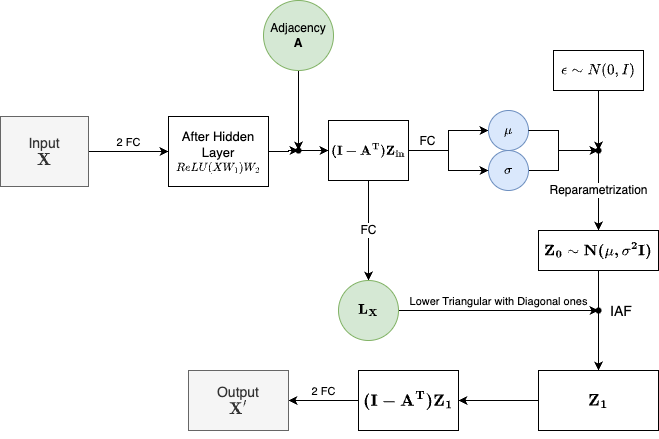
\includegraphics[width=0.8\textwidth]{fig/model.png}
    \caption{Architecture of the proposed model.}
    \label{diagram}
\end{figure}

\subsection{Learning}

Our model aims to learn the adjacency matrix of the directed acyclic graph. Instead of regarding the mixed graph as a cyclic graph, we consider them as DAG structure with correlated noise variables. Thus we can use the same optimization procedure as DAG-GNN, which uses the acyclicity constraint as a continuous approximation of the discrete constraint. The optimization procedure is minimizing the following loss function:

\begin{equation}
    \mathcal{L}(A, W, \lambda) =-\mathcal{L}_{\mathrm{ELBO}} + \tau_A \Vert A \Vert_1 + \lambda h(A) + \frac{c}{2} |h(A)|^2.
\end{equation}

The second term is the L1 regularization term, which encourages sparsity of the adjacency matrix. The third and fourth terms are the augmented Lagrangian terms. Since larger value of $c$ makes the acyclicity constraint to zero, the training process is done by gradually increasing the value of $c$. \cite{yu2019daggnn}\\





\section{Experiment}

In this section, we conduct experiments on simulated data to evaluate the performance of our proposed method. We compare our method with the DAG-GNN \cite{yu2019daggnn} with random graph datasets. We used a thresholding value of extracting graph as 0.3 which is the same value used at DAG-GNN and NOTEARS.\\ 

\paragraph*{Datasets} Random graph datasets are generated using the following procedure. First, we generate a random directed acyclic graph using the Erdős–Rényi model. In Section 5.1, we conduct experiments where the noise variables follows a multivariate Gaussian distribution with a non-diagonal covariance matrix. We randomly select a given proportion of edges and make them bidirectional. Then, we generate a corresponding random covariance matrix and generate multivariate Gaussian data using that covariance matrix. We generate 5000 samples for each graph. For the size of the graph, we use 10, 20, 30, and 50 nodes. For the proportion of bidirectional edges, we use 0, 0.1, 0.3, 0.5, and 0.8. In Section 5.2, we consider the case where the noise variables follow not only an independent Gaussian distribution but also independent Laplace and exponential distributions.\\

\paragraph*{Evaluation} We evaluate the performance of our method using two metrics: Structural Hamming Distance (SHD) and False Discovery Rate (FDR). SHD measures the number of edge additions, deletions, and reversals required to transform the estimated graph into the true graph. FDR represents the ratio of false positives to the total number of predicted edges. These metrics are calculated by comparing the estimated graph with the true graph, considering bidirectional edges. For each combination of the number of nodes and the proportion of bidirectional edges, we generate at least 5 random graphs and calculate the average metrics.

\subsection{Independent Noise Case}

Here is the introduction of our experiment on independent noise case

\subsection{Dependent Noise Case}

Here is the introduction of our experiment on dependent noise case

\section{Conclusion}

Here is the conclusion

% Biblography
\bibliographystyle{ieeetr}
\bibliography{references}

\end{document}

